\section{Asimov B \deltacp/mass-hierarchy degeneracy}
\label{app:asimovb_sensitivity}

In \cref{sec:sensitivity:asimov_results} it was noted that Asimov B fits are affected by a lack of sensitivity to distinguish $\delta_{CP} = 0$ and $\delta_{CP} = \pi$, for example, the fit of \deltacp shown in \cref{fig:ssqth13_vs_dcp_sensitivity} shows a best-fit point shifted away from the true value. \cref{fig:asimovb_spectra_degeneracy} shows normalised one-ring $e$-like spectra for Asimov data set B with mass hierarchy and \deltacp varied to demonstrate the problem. It is clear from the plots that the spectrum for $\delta_{CP} = 0$ in normal hierarchy is similar in shape to the spectrum for $\delta_{CP} = \pi$ in inverted hierarchy and vice versa.

\begin{figure*}[htb]
	\begin{subfigure}[b]{0.49\textwidth}
		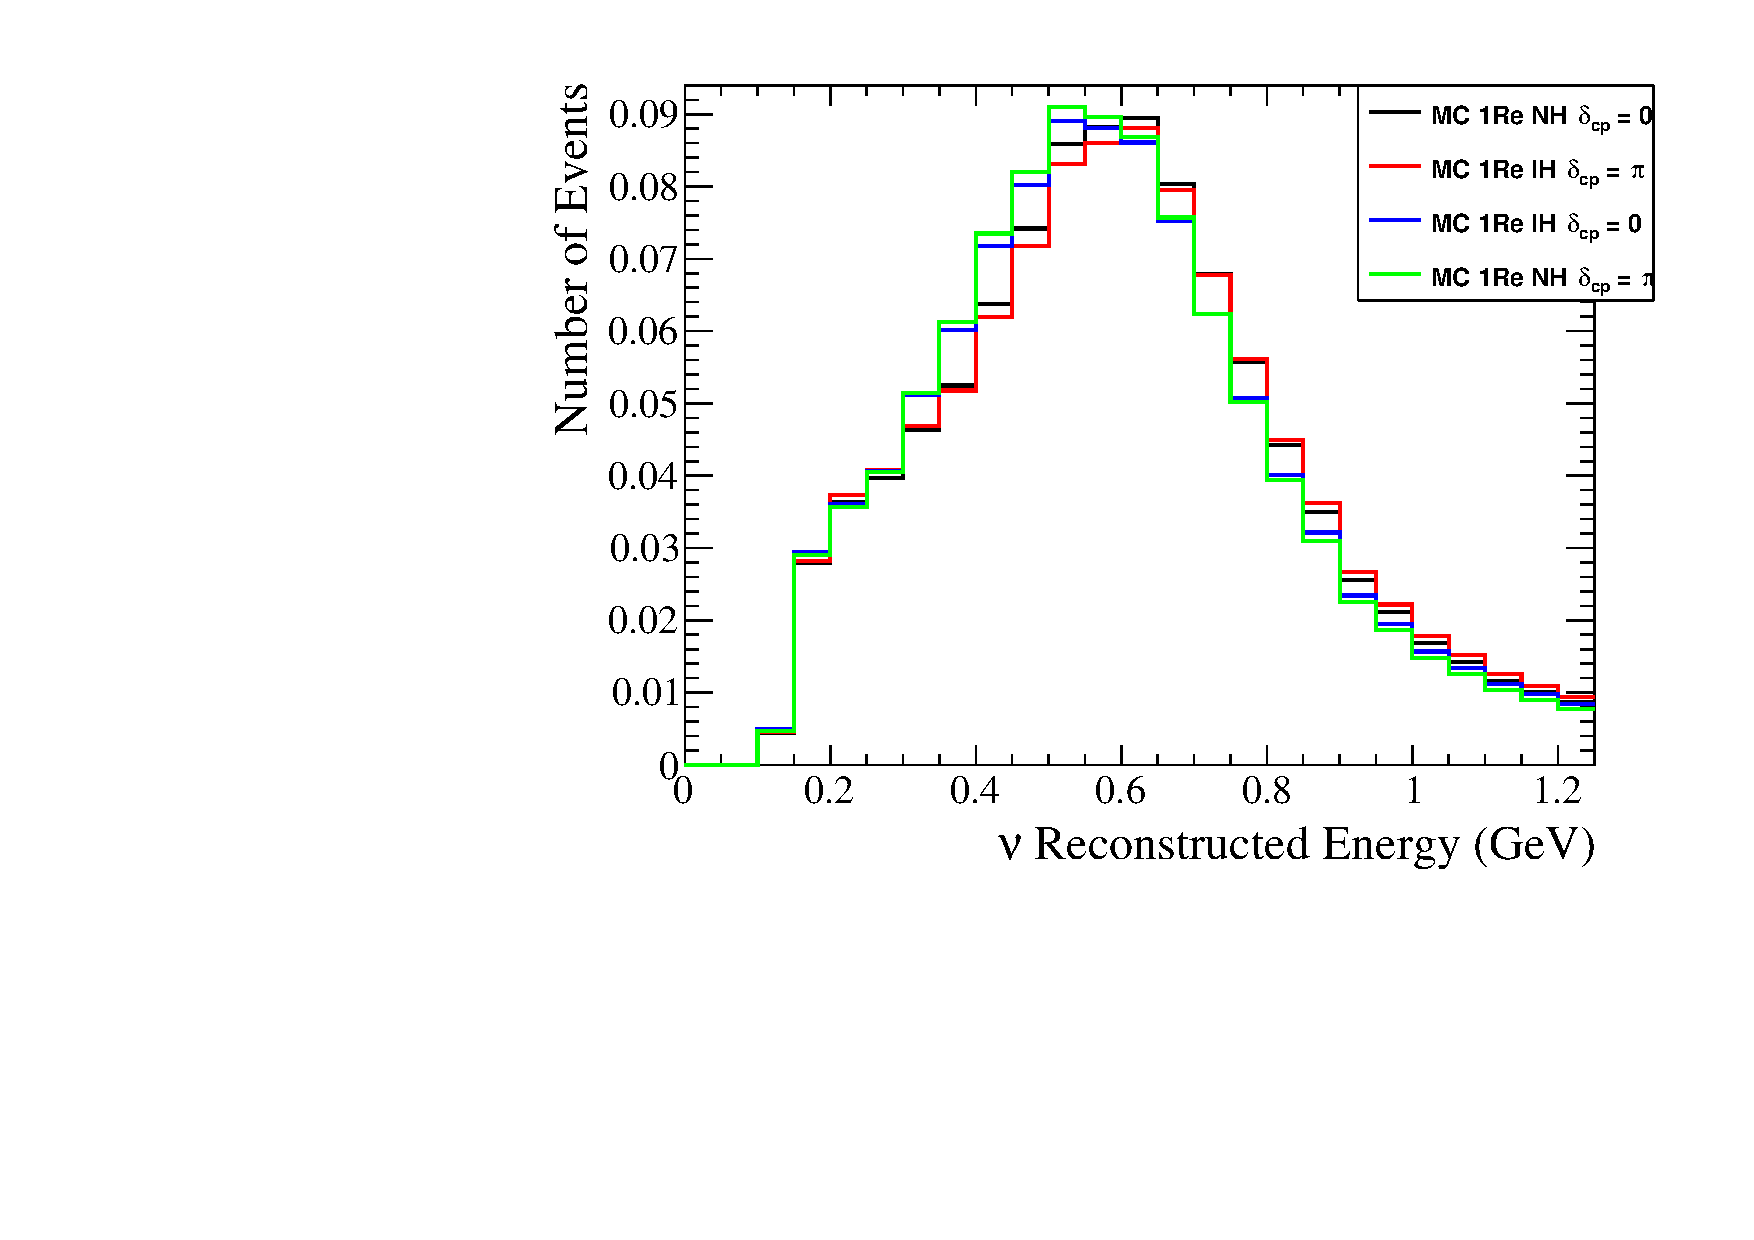
\includegraphics[width=0.9\textwidth]{images/spectra/asimovb_degeneracy_fhc}
		\caption{MC one-ring FHC $e$-like spectra}
	\end{subfigure}
	\begin{subfigure}[b]{0.49\textwidth}
		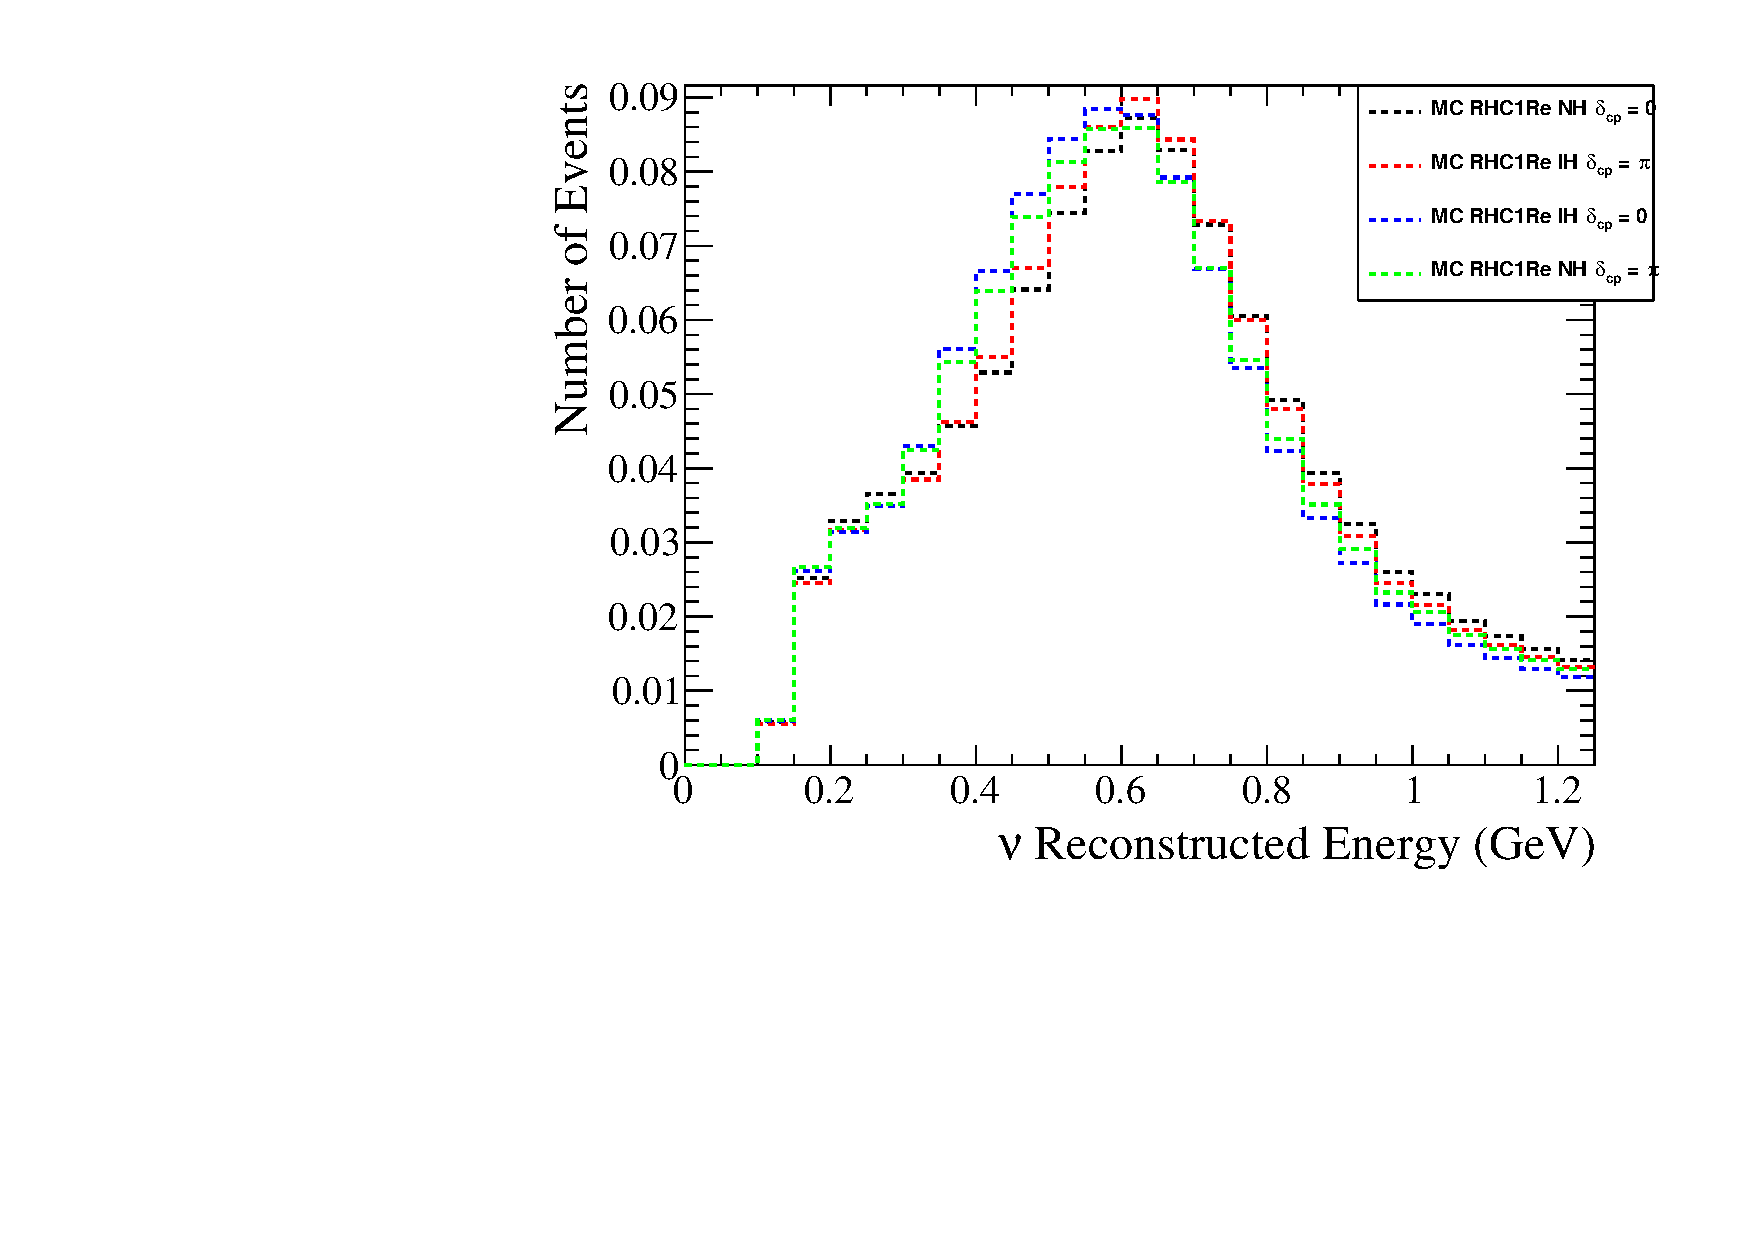
\includegraphics[width=0.9\textwidth]{images/spectra/asimovb_degeneracy_rhc}
		\caption{MC one-ring RHC $e$-like spectra}
	\end{subfigure}
	\caption {
		Normalised spectra for one-ring $e$-like samples showing the effect of changing the mass hierarchy and true value of \deltacp for the Asimov B data set.
	}
	\label{fig:asimovb_spectra_degeneracy}
\end{figure*}
\clearpage